\documentclass[12pt]{article}
\usepackage{amssymb,amsmath,latexsym, braket}
\usepackage{tikz, pgfplots, graphicx, standalone}
\newcommand{\dt}[1]{\frac{\mathrm d #1}{\mathrm dt}}
%\usetikzlibrary{external}
%\tikzexternalize[prefix=i/]
\begin{document}

\title{The Kuramoto Model}
\author{Manish Goregaokar}

\maketitle

\begin{abstract}
Synchronization is a common phenomenon occurring with coupled oscillators, where over time their phases become locked. It is observed in a wide range of situations, from the tidal locking of the moon to neural clusters. This report gives an overview of this phenomenon, with specific focus on the Kuramoto model.
\end{abstract}
\tableofcontents
\section{Introduction}

In 1665, Christian Huygens made the first recorded observation and analysis of synchronization\cite{bennett2002huygens}. He noticed that a pair of pendulums kept in the same housing would gradually start moving in unison regardless of their initial conditions. Additionally, if perturbed after the synchronization, the pendulums would re-synchronize. He attributed this effect to the motion of the beam connecting the two, but did not manage to make a complete model of this phenomenon.

The field was quite dormant until the early 1900s, when J. Vincent\cite{vincent1919some}, Van Der Pol\cite{van1920theory}, and E. Appleton\cite{appleton1922automatic} experimented with electrical circuits involving triode oscillators.

After this, there has been a myriad of topics in which synchronization has been studied, including in many electrical, chemical, and biological systems. Additionally, the phenomenon has many applications --- for example, pacemakers are a driving oscillator to the heart in a synchronized system.

\section{Basics}
\subsection{Coupled oscillators}
Systems which individually behave as oscillators can be "coupled", such that at least one of them is exposed to an effect dependent on the phases of the two oscillators. Usually this effect is monotonic and dependent on the phase difference only. Coupling can be one way or two way ("mutual coupling"). In the one-way case we have a "driving oscillator" which is unaffected by the other oscillator(s), and the other oscillator(s) are known as the "driven oscillator(s)".

For example, for a pair of oscillators, unidirectional coupling could have the equations:
\begin{align*}
\dt{\phi_1} &= \omega \\
\dt{\phi_2} &= \omega - k\sin(\phi_2 - \phi_1)
\end{align*}

whereas bidirectional coupling would be:
\begin{align*}
\dt{\phi_1} &= \omega + k\sin(\phi_2 - \phi_1)\\
\dt{\phi_2} &= \omega - k\sin(\phi_2 - \phi_1)
\end{align*}

In cases where one oscillator has no external effects, sometimes it is considered as ``external forcing".


Oscillators need not have the same $\omega$ (or in general, the same state-space portraits) to be coupled.

\subsection{Synchronization}
TODO
\subsection{Ensemble of oscillators}
\begin{figure}
\centering
\includestandalone[mode=image]{i/almostfull}
\caption{Almost full synchronization}\label{fig:fullgraph}
\end{figure}

\begin{figure}
\centering
\includestandalone[mode=image]{i/partial}

\caption{Partial synchronization}\label{fig:partialgraph}
\end{figure}

\begin{figure}
\centering
\includestandalone[mode=image]{i/nonesync}

\caption{No synchronization}\label{fig:nograph}
\end{figure}
Typically, most synchronizing real systems can be modeled with an \emph{ensemble} of coupled oscillators. Coupling may or may not be global.

In such an ensemble, synchronization can be "partial"; i.e. there are some elements of synchronization to be found, but it is still not fully synchronized. For example, in Figure \ref{fig:fullgraph}, we have the time series for a system of almost completely synchronized oscillators (Complete full synchronization would be where the time series for all oscillators are equal or opposite).

Contrast this with Figure \ref{fig:nograph}, where there is no synchronization at all. While there are times in which the oscillators seem to come close to synchronization, these do not last. However, in Figure \ref{fig:partialgraph}, we have what is known as ``partial synchronization". The majority of the oscillators here are close to the ``mean" timesemble of coupled oscillators
$$\dot{\theta_i} = \omega_i + \frac{K}{N}\sum_j a_{ij}\sin(\theta_j - \theta_i) $$
 series, though there may be a minority of oscillators which are out of phase. It is not necessary that the \emph{sames} oscillators will continue to stay somewhat in phase; usually the number of partially synchronized oscillators is approximately constant, however individual oscillators alternate between being in phase and out of phase with the rest.



\section{The Kuramoto Model}
TODO intro
The Kuramoto model models an ensemble of coupled oscillators
$$\dot{\theta_i} = \omega_i + \frac{K}{N}\sum_j a_{ij}\sin(\theta_j - \theta_i) $$

Here, $N$ is the number of oscillators, $K$ is the coupling parameter, and $a_{ij}$ determines how the network of oscillators is coupled. Usually, $a_{ij}=a_{ji}$, and its value is either 0 or 1, denoting uncoupled and coupled oscillators respectively. Interesting behavior can be observed when the $\omega_i$s are different

\subsection{Order parameter}
An important way to measure the ``amount" of synchronization. is via something known as the \emph{order parameter}. For an ensemble of oscillators with phases $\theta_i$, the Kuramoto order parameter is 

$$r = \frac1{N}\left|\sum_i e^{i\theta_i}\right|$$

For a completely synchronized system, this parameter is 1, and for an unsynchronized system it will usually be a low value. Partial synchronization is when the value is not small on an average.
\subsection{Analysis of a globally coupled Kuramoto system}
\begin{figure}
\centering
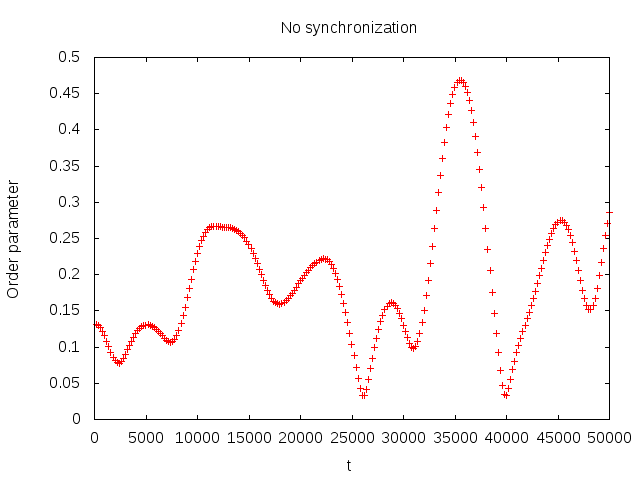
\includegraphics[scale=0.5]{data/strange}
\caption{No synchronization with $K=0.01$}
\label{fig:plot:nosynchro}
\end{figure}

I simulated a globally coupled Kuramoto system of 30 oscillators, with a 10\% variation in the $\omega_i$s, and varied $K$. For very low $K$, we get no synchronization as seen in Figure \ref{fig:plot:nosynchro}. While the order parameter may rise to larger values (sometimes even coming close to 1), \emph{on an average} the order parameter stays very low.

While in some cases for partial synchronization the order parameter settles on a particular value and doesn't vary (Figure \ref{fig:plot:partial2}), this is not true in the general case. For example, for lower values of $K$ we can get a time evolution like in Figure \ref{fig:plot:partial1}, where
\begin{figure}
\centering
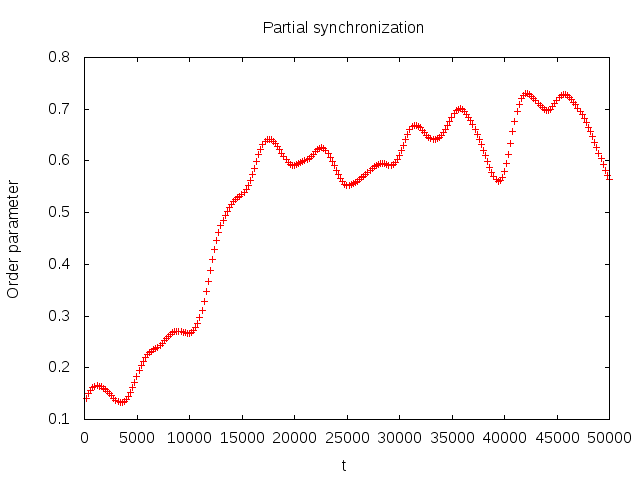
\includegraphics[scale=0.5]{data/partialsm}
\caption{Partial synchronization with $K=0.05$}
\label{fig:plot:partial1}
\end{figure}

\begin{figure}
\centering
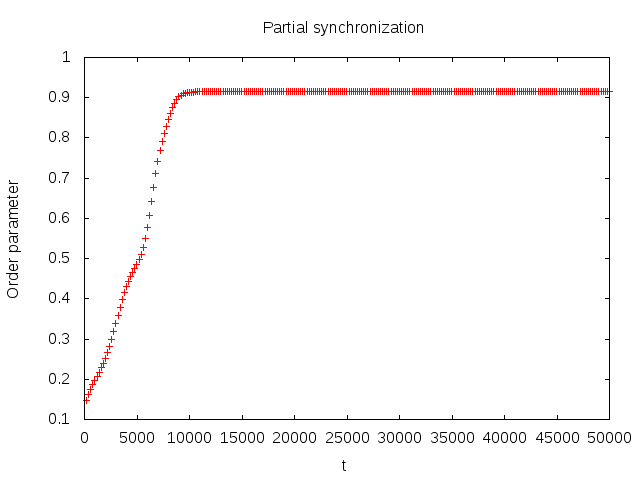
\includegraphics[scale=0.5]{data/partialmore}
\caption{Partial synchronization with $K=0.07$}
\label{fig:plot:partial2}
\end{figure}

\begin{figure}
\centering
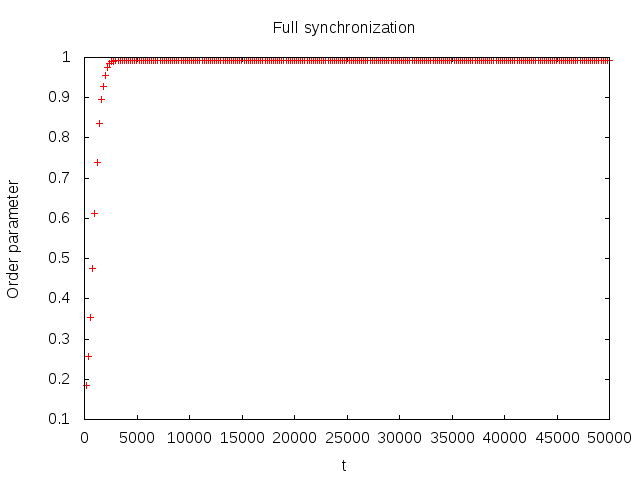
\includegraphics[scale=0.5]{data/full}
\caption{Full synchronization with $K=0.2$}
\label{fig:plot:full1}
\end{figure}

\bibliographystyle{abbrv}
\bibliography{bib}

\end{document}